%!TEX root = ../Thesis.tex
%% Basierend auf TeXnicCenter-Vorlage von Mark Müller
%%                      Willi Nüßer
%%                      Waldemar Penner     
%%                      Ulrich Reus
%%                      Frank Plass
%%                      Oliver Tribeß 
%%                      Daniel Hintze     
%%%%%%%%%%%%%%%%%%%%%%%%%%%%%%%%%%%%%%%%%%%%%%%%%%%%%%%%%%%%%%%%%%%%%%%

% Wählen Sie die Optionen aus, indem Sie % vor der Option entfernen  
% Dokumentation des KOMA-Script-Packets: scrguide

%%%%%%%%%%%%%%%%%%%%%%%%%%%%%%%%%%%%%%%%%%%%%%%%%%%%%%%%%%%%%%%%%%%%%%%
%% Optionen zum Layout des Artikels                                  %%
%%%%%%%%%%%%%%%%%%%%%%%%%%%%%%%%%%%%%%%%%%%%%%%%%%%%%%%%%%%%%%%%%%%%%%%
\documentclass[%
paper=A4,         % alle weiteren Papierformat einstellbar
fontsize=12pt,    % Schriftgröße (12pt, 11pt (Standard))
BCOR=12mm,         % Bindekorrektur, bspw. 1 cm
DIV=14,            % breiter Satzspiegel
parskip=half*,    % Absatzformatierung s. scrguide 3.1
headsepline,      % Trennline zum Seitenkopf  
%footsepline,     % Trennline zum Seitenfuß
%normalheadings,  % Überschriften etwas kleiner (smallheadings)
listof=totoc,     % Tabellen & Abbildungsverzeichnis ins Inhaltsverzeichnis      
%bibtotoc,        % Literaturverzeichnis im Inhalt 
%draft            % Überlangen Zeilen in Ausgabe gekennzeichnet
footinclude=false,% Fußzeile in die Satzspiegelberechnung einbeziehen 
headinclude=true, % Kopfzeile in die Satzspiegelberechnung einbeziehen 
final             % draft beschleunigt die Kompilierung
]
{scrartcl}

%\setuptoc{toc}{totoc} % Inhaltsverzeichnis ins Inhaltsverzeichnis

% Neue Deutsche Rechtschreibung und Deutsche Standardtexte
\usepackage[ngerman]{babel} 

% Umlaute können verwendet werden
\usepackage[utf8]{inputenc}   

% Echte Umlaute
\usepackage[T1]{fontenc} 

% Latin Modern Font, Type1-Schriftart für nicht-englische Texte
\usepackage{lmodern} 

% 1/2-zeiliger Zeilenabstand
\usepackage[onehalfspacing]{setspace}

% Für die Defenition eigener Kopf- und Fußzeilen
\usepackage{fancyhdr} 

% Für die Verwendung von Grafiken
\usepackage[pdftex]{graphicx}

% Bessere Tabellen
\usepackage{tabularx}

% Für die Befehle \toprule, \midrule und \bottomrule, z.B. in Tabellen 
\usepackage{booktabs}

% Erlaubt die Benutzung von Farben
\usepackage{color}

% Verbessertes URL-Handling mit \url{http://...}
\usepackage{url}

% Listen ohne Abstände \begin{compactlist}...\end{compactlist}
\usepackage{paralist} 

% Ausgabe der aktuellen Uhrzeit für die Draft-Versionen
\usepackage{datetime}

% Deutsche Anführungszeichen
\usepackage[babel,german=quotes]{csquotes}

\usepackage{xcolor}

\usepackage{float} % For [H] option#

\usepackage{minted}

% Konfiguration der Abbildungs- und Tabellenbezeichnungen
\usepackage[format=hang, font={footnotesize, sf}, labelfont=bf, justification=raggedright,singlelinecheck=false]{caption}

% Verbessert die Lesbarkeit durch Mikrotypografie
\usepackage[activate={true,nocompatibility},final,tracking=true,kerning=true,spacing=true,factor=1100,stretch=10,shrink=10]{microtype}  

% Zitate und Quellenverzeichnis
\usepackage[
    bibstyle=authoryear,
    citestyle=authoryear-fhdw,  
    giveninits=false,         % false = Vornamen werden ausgeschrieben
    natbib=true,
    urldate=long,             % "besucht am" - Datum
    %url=false,
    date=long,                
    dashed=false, 
    maxcitenames=3,           % max. Anzahl Autorennamen in Zitaten
    maxbibnames=99,           % max. Anzahl Autorennamen im Quellenverzeichnis
    %backend=bibtex           % Ggf. für ältere Distributionen bibtex verwenden
    backend=biber
]{biblatex}
  
% Bibliograpthy
% \bibliography{library/library}
\addbibresource{library/library.bib}  % Your.bib file

% Keine Einrückung bei einem neuen Absatz 
\parindent 0pt 

% Ebenentiefe der Nummerierung
\setcounter{secnumdepth}{3}

% Gliederungstiefe im Inhaltsverzeichnis 
\setcounter{tocdepth}{3} 

% Tabellen- und Abbildungsverzeichnis mit Bezeichnung:
\usepackage[titles]{tocloft}

% Sourcecode-Listings
\usepackage{listings}

% Bestimmte Warnungen unterdrücken
% siehe http://tex.stackexchange.com/questions/51867/koma-warning-about-toc
\usepackage{scrhack} 

%% http://tex.stackexchange.com/questions/126839/how-to-add-a-colon-after-listing-label
\makeatletter
\begingroup\let\newcounter\@gobble\let\setcounter\@gobbletwo
  \globaldefs\@ne \let\c@loldepth\@ne
  \newlistof{listings}{lol}{\lstlistlistingname}
\endgroup
\let\l@lstlisting\l@listings
\makeatother

\renewcommand*\cftfigpresnum{Abbildung~}
\renewcommand*\cfttabpresnum{Tabelle~}
\renewcommand*\cftlistingspresnum{Listing~}
\renewcommand{\cftfigaftersnum}{:}
\renewcommand{\cfttabaftersnum}{:}
\renewcommand{\cftlistingsaftersnum}{:}
\settowidth{\cftfignumwidth}{\cftfigpresnum 99~\cftfigaftersnum}
\settowidth{\cfttabnumwidth}{\cfttabpresnum 99~\cftfigaftersnum}
\settowidth{\cftlistingsnumwidth}{\cftlistingspresnum 99~\cftfigaftersnum}
\setlength{\cfttabindent}{1.5em}
\setlength{\cftfigindent}{1.5em}
\setlength{\cftlistingsindent}{1.5em}

\renewcommand\lstlistlistingname{Listingverzeichnis}
 
% Style für Kopf- und Fußzeilenfelder
\pagestyle{fancy}
\fancyhf{}
\fancyhead[R]{\leftmark}
\fancyfoot[R]{\thepage} 
\renewcommand{\sectionmark}[1]{\markboth{#1}{#1}} 
\fancypagestyle{plain}{}

% Macro für Quellenangaben unter Abbildungen und Tabellen
\newcommand{\source}[1]{{\vspace{-1mm}\\\footnotesize\textsf{\textbf{Quelle:}} \textsf{#1}\par}}

% Anpassungen der Formatierung an Eclipse-Aussehen 
% http://jevopi.blogspot.de/2010/03/nicely-formatted-listings-in-latex-with.html
%\definecolor{sh_comment}{rgb}{0.12, 0.38, 0.18 } %adjusted, in Eclipse: {0.25, 0.42, 0.30 } = #3F6A4D
%\definecolor{sh_keyword}{rgb}{0.37, 0.08, 0.25}  % #5F1441
%\definecolor{sh_string}{rgb}{0.06, 0.10, 0.98} % #101AF9
% Für Druckausgabe sollte alles schwarz sein
\definecolor{sh_comment}{rgb}{0.0, 0.0, 0.0 }
\definecolor{sh_keyword}{rgb}{0.0, 0.0, 0.0 }
\definecolor{sh_string}{rgb}{0.0, 0.0, 0.0 }

\lstset{ %
  language=Java,
  basicstyle=\small\ttfamily,
  fontadjust, 
  xrightmargin=1mm,
  xleftmargin=5mm,
  tabsize=2,
  columns=flexible,
  showstringspaces=false,
  rulesepcolor=\color{black},
  showspaces=false,showtabs=false,tabsize=2,
  stringstyle=\color{sh_string},
  keywordstyle=\color{sh_keyword}\bfseries,
  commentstyle=\color{sh_comment}\itshape,
  captionpos=t,
  lineskip=-0.3em
}

%\makeatletter
%\def\l@lstlisting#1#2{\@dottedtocline{1}{0em}{1.5em}{\lstlistingname\space{#1}}{#2}}
%\makeatother

% Anhangsverzeichnis
\usepackage[nohints]{minitoc} %Anhangsverzeichnis

\makeatletter
\newcounter{fktnr}\setcounter{fktnr}{0}
\newcounter{subfktnr}[fktnr]\setcounter{subfktnr}{0}

\renewcommand\thesubfktnr{\arabic{fktnr}.\arabic{subfktnr}}
\newcounter{anhangcounter}
\newcommand{\blatt}{\stepcounter{anhangcounter}}

\newcommand{\anhang}[1]{\setcounter{anhangcounter}{0}\refstepcounter{fktnr}
\addcontentsline{fk}{subsection}{Anhang~\thefktnr: \hspace*{1em}#1}
\subsection*{{Anhang~\thefktnr \hspace*{1em} #1 \hspace*{-1em}}}
}

\newcommand{\subanhang}[1]{\setcounter{anhangcounter}{0}\refstepcounter{subfktnr}
\addcontentsline{fk}{subsubsection}{Anhang~\thesubfktnr: \hspace*{1em}#1}
\subsubsection*{{Anhang~\thesubfktnr \hspace*{1em} #1 \hspace*{-1em}}}
}

\newcommand{\anhangsverzeichnis}{\mtcaddsection{\subsection*{Anhangsverzeichnis \@mkboth{FKT}{FKT}}}\@starttoc{fk}\newpage}

% Links im PDF
\usepackage[pdfpagemode={UseOutlines}, plainpages=false,breaklinks=true,pdfpagelabels]{hyperref}

 % Abkürzungsverzeichnis
\usepackage[automake,
			acronym,         % create list of acronyms
            nonumberlist,
            toc, 
            section,
            nopostdot,  % avoid dot after acronym
            hyperfirst=false,% don't hyperlink first use
            %sanitize=none    % switch off sanitization as description % Deprecated
            ]{glossaries}
            \newglossarystyle{mylist}{%
\setglossarystyle{long}% base this style on the list style
\renewcommand*{\glossaryentryfield}[5]{%
    \glsentryitem{##1}\textbf{##2} & ##3 \\}%
}

% Verbessert das Referenzieren von Kapiteln, Abbildungen etc.
\usepackage[german,capitalise]{cleveref}

\makeglossaries\makeglossaries 
%Acronyms
\newacronym{AES}{AES}{Advanced Encryption Standard}
\newacronym{AI}{AI}{Artificial Intelligence}
\newacronym{AOA}{AOA}{Angle of Arrival}
\newacronym{API}{API}{Application Programming Interface}
\newacronym{ATM}{ATM}{Automated Teller Machine}

%Glossary
\newglossaryentry{Glossar}
{
	name=Glossar,
	description={Ein Glossar ist eine alphabetisch geordnete Liste von Begriffen aus einem bestimmten Wissensgebiet mit den dazugehörigen Definitionen.}
}



%%%%%%%%%%%%%%%%%%%%%%%%%%%%%%%%%%%%%%%%%%%%%%%%%%%%%%%%%%%%%%%%%%%%%%%
%% Parameter - Hier auf die eigene Arbeit anpassen
%%%%%%%%%%%%%%%%%%%%%%%%%%%%%%%%%%%%%%%%%%%%%%%%%%%%%%%%%%%%%%%%%%%%%%%

\newcommand{\studiengang}{Wirtschaftsinformatik} 
\newcommand{\spezialisierungsbereich}{Cyber Security}	
\newcommand{\martikelnummer}{101485}
\newcommand{\dokumententyp}{Praxisarbeit}
\newcommand{\abgabedatum}{26.08.2024} 
\newcommand{\ort}{Langenfeld} 
\newcommand{\koorperationsunternehmen}{Bayer AG}
\newcommand{\fhdwstandort}{Bergisch Gladbach} % oder Bielefeld, Mettmann, ...
\newcommand{\dokumententitel}{Observability und Monitoring von AWS-Prozessen}
\newcommand{\dokumentenautor}{Thomas Benjamin Hopf}
\newcommand{\dokumentenautoradress}{Heinrichstraße 23, 40764 Langenfeld}
\newcommand{\dokumentenpruefer}{Prof. Dr. Christian Soltenborn}

%%%%%%%%%%%%%%%%%%%%%%%%%%%%%%%%%%%%%%%%%%%%%%%%%%%%%%%%%%%%%%%%%%%%%%%

\hypersetup{
  colorlinks=false,
  pdfborder={0 0 0},
  pdftitle=\dokumententitel,
  pdfauthor=\dokumentenautor
} 

\begin{document}

% Römische Seitennummerierung
\pagenumbering{Roman}
 
%%%%%%%%%%%%%%%%%%%%%%%%%%%%%%%%%%%%%%%%%%%%%%%%%%%%%%%%%%%%%%%%%%%%%%%
%% Titelseite
%%%%%%%%%%%%%%%%%%%%%%%%%%%%%%%%%%%%%%%%%%%%%%%%%%%%%%%%%%%%%%%%%%%%%%%

%!TEX root = ../Thesis.tex

\begin{titlepage}

\begin{center}

\includegraphics[scale=0.8]{img/fhdw}

\vspace{7mm}

\Huge{\bfseries\dokumententyp}\\

\vspace{5mm}

\LARGE{\dokumententitel}\\

\vspace{15mm}

\large{Prüfer(in):\\

\dokumentenpruefer\\

\vspace{15mm}

Verfasser(in):\\

\dokumentenautor\\

\martikelnummer\\

\vspace{3mm}

\dokumentenautoradress\\

\vspace{7mm}

\studiengang\\

\spezialisierungsbereich\\

}

\enlargethispage{2em}

\vspace{15mm}

\large{Eingereicht am:\\

\abgabedatum \\

}

\end{center}


\end{titlepage}



%%%%%%%%%%%%%%%%%%%%%%%%%%%%%%%%%%%%%%%%%%%%%%%%%%%%%%%%%%%%%%%%%%%%%%%
%% Draft-Einstellungen
%%
%% Für die finale Version auskommentieren!
%%%%%%%%%%%%%%%%%%%%%%%%%%%%%%%%%%%%%%%%%%%%%%%%%%%%%%%%%%%%%%%%%%%%%%%
%%\fancyhead[L]{\color{red} Stand: \today~-~\currenttime}

%%%%%%%%%%%%%%%%%%%%%%%%%%%%%%%%%%%%%%%%%%%%%%%%%%%%%%%%%%%%%%%%%%%%%%%
%% Verzeichnisse
%%%%%%%%%%%%%%%%%%%%%%%%%%%%%%%%%%%%%%%%%%%%%%%%%%%%%%%%%%%%%%%%%%%%%%%


% Sperrvermerk
%!TEX root = ../Thesis.tex
\section*{Sperrvermerk}
\addcontentsline{toc}{section}{Sperrvermerk}
\fancyhead[R]{Sperrvermerk}

Diese Arbeit enthält vertrauliche Informationen über die Firma \koorperationsunternehmen. Die Weitergabe des Inhalts dieser Arbeit (auch in Auszügen) ist untersagt. Es dürfen keinerlei Kopien oder Abschriften - auch nicht in digitaler Form - angefertigt werden. Auch darf diese Arbeit nicht veröffentlicht werden und ist ausschließlich den Prüfern, Mitarbeitern der Verwaltung und Mitgliedern des Prüfungsausschusses sowie auf Nachfrage einer Evaluierungskommission zugänglich zu machen. Personen, die Einsicht in diese Arbeit erhalten, verpflichten sich, über die Inhalte dieser Arbeit und all ihren Anhängen keine Informationen, die die Firma \koorperationsunternehmen{} betreffen, gegenüber Dritten preiszugeben. Ausnahmen bedürfen der schriftlichen Genehmigung der Firma \koorperationsunternehmen{} und des Verfassers.


Die Arbeit oder Teile davon dürfen von der FHDW einer Plagiatsprüfung durch einen Plagiatsoftware-Anbieter unterzogen werden. Der Sperrvermerk ist somit im Fall einer Plagiatsprüfung nicht wirksam.
\newpage
\fancyhead[R]{\leftmark}

% Inhaltsverzeichnis
\tableofcontents\newpage

% Glossar
\renewcommand{\glossarypreamble}{\label{glossary}}
\printglossary[style=long, title=Glossar, toctitle=Glossar] \newpage

% Abkürzungsverzeichnis
\renewcommand{\glossarypreamble}{\label{acronyms}}
\printglossary[type=acronym, style=long, title=Abkürzungsverzeichnis, toctitle=Abkürzungsverzeichnis] \newpage

\setcounter{table}{0} % printglossary erzeugt eine Tabelle, die die Nummerierung der "echten" Tabellen durcheinander bringt.

%%%%%%%%%%%%%%%%%%%%%%%%%%%%%%%%%%%%%%%%%%%%%%%%%%%%%%%%%%%%%%%%%%%%%%%
% Verzeichnisse
%%%%%%%%%%%%%%%%%%%%%%%%%%%%%%%%%%%%%%%%%%%%%%%%%%%%%%%%%%%%%%%%%%%%%%%

% Abbildungsverzeichnis
\fancyhead[R]{\listfigurename}
\listoffigures\newpage

% Tabellenverzeichnis
\fancyhead[R]{\listtablename}
\listoftables\newpage

% Quelltextverzeichnis
\fancyhead[R]{\lstlistlistingname}
%\lstlistoflistings\newpage

% Kapitelüberschriften für den Arbeitstext
\fancyhead[R]{\leftmark}

%%%%%%%%%%%%%%%%%%%%%%%%%%%%%%%%%%%%%%%%%%%%%%%%%%%%%%%%%%%%%%%%%%%%%%%
%% Inhalt
%%%%%%%%%%%%%%%%%%%%%%%%%%%%%%%%%%%%%%%%%%%%%%%%%%%%%%%%%%%%%%%%%%%%%%%

% Arabische Seitennummerierung
\pagenumbering{arabic} 

\section{Einleitung und Motivation}
Die Mitarbeiter der Fachabteilungen benutzen eine in AWS aufgebaute API, um auf betriebsrelevante Daten zuzugreifen. Die Reliabilität dieser API ist dementsprechend betrieblich wichtig. Die Hintergrundprozesse in der Datenverarbeitung und Bereitstellung sind jedoch nicht einsichtig; wird eine Information aus einem Datensatz angefordert, lässt sich nur einsehen, ob der Prozess korrekt abgelaufen ist oder nicht. Fehlerdetails werden nicht übermittelt, wodurch die Identifizierung und Behebung von Fehlern nur schwer möglich ist. Zudem ist bisher keine Oberfläche implementiert, mit der die Antwortgeschwindigkeit (im Folgenden ``Response time'') im zeitlichen Kontext überwacht werden kann. Diese beiden Faktoren wirken sich negativ auf die Effizienz und Effektivität der API aus, weshalb die in der Zielsetzung beschriebene Lösung implementiert werden soll.
\subsection{Zielsetzung}
Im Rahmen dieser Praxisarbeit soll die Effizienz  und Effektivität der API gesteigert werden, indem Fehlerinformationen transparent gestaltet werden und die Möglichkeit der Überwachung der Response time geschaffen werden. Für die Dokumentation der Fehler soll die Applikation ``CloudWatch'' Einsicht in die Prozesse geben. Zusätzlich soll die Auftrittshäufigkeit von Fehlern in einem Dashboard dargestellt werden. Die Überwachung der Response time über die Zeit soll durch die Applikation „WatchDog“ erreicht werden. Hierzu sollen relevante Daten zu den jeweiligen Anfragen gesammelt und dargestellt werden, sodass auch Trends erkennbar sind. 
\subsection{Aufbau der Arbeit}
Zuerst sollen die Konzepte und Werkzeuge geklärt werden, mit denen in der Arbeit gearbeitet wird. Dann sollen die konkreten Anforderungen definiert werden, die aus der Zielsetzung hervorgehen. Dann soll die Umsetzung dieser Anforderungen erläutert werden.  
\subsection{Unternehmen}
Bayer, gegründet 1863 als „Friedr. Bayer et comp.“ , mit Sitz in Leverkusen ist das weltweit umsatzstärkste Unternehmen im Bereich CropScience. Aufgeteilt ist das Unternehmen in drei Divisionen: Pharmaceuticals, also der Herstellung verschreibungspflichtiger Arzneimittel, Consumer Health, die Herstellung sogenannter „Over-the-Counter Medikamente“, für welche keine ärztliche Verschreibung nötig ist, und CropScience, der Pflanzenschutzdivision. Zusätzlich zu den drei Divisionen existieren die „Enabling Functions“. Diese unterstützen das Tagesgeschäft, sind aber keiner der Divisionen direkt untergeordnet, sondern stehen neben den Divisionen und unterstützen diese. Diese Praxisarbeit behandelt ein Projekt, welches primär für Crop-Science Nutzer relevant ist, jedoch im Auftrag einer Abteilung der „Enabling Functions“ durchgeführt wird. Für die Enabling Function ist Effizienz und Effektivität ein wichtiges Kriterium, woraus sich die Relevanz dieser Arbeit ableitet.
\subsection{Relevanz für das Unternehmen}
Neben den geringeren Prozesskosten in der Verantwortung der Enabling Functions führt eine gesteigerte Effizienz und Effektivität zu einer verbesserten Nutzerfreundlichkeit. Durch Benachrichtigungen können Fehler schneller behoben werden, wodurch die Uptime erhöht wird und durch Monitoring der Response time kann entsprechend bei negativen Trends dieser früher gehandelt werden. Dadurch soll die API schlussendlich, gestützt von den zu implementierenden Anwendungen, zuverlässiger laufen und zu verbessertem Nutzerempfinden führen.
\subsection{Einschränkung}
Aus zeitlichen Gründen wird im Rahmen dieser Praxisarbeit die Implementierung nur auf einem Test-System durchgeführt, und alle beschriebenen Komponenten sind nur für Testzwecke aufgebaut. Die Daten haben dementsprechend nicht immer semantische Relevanz, solange eine solche keinen Einfluss auf die Feststellung der Funktionalität der Infrastruktur haben. Die Anwendungen, mit denen im Rahmen dieser Praxisarbeit gearbeitet wird, sind Teil der Standard-Suite der Abteilung, die den Auftrag für diese Arbeit erteilt hat. Es hat keine eigene Auswahl bei diesen Anwendungen stattgefunden, weshalb die Auswahl der Anwendungen auch kein Thema in dieser Arbeit ist.
\section{Grundlagen}
In diesem Projekt wird ein Testsystem von Grund auf aufgebaut, mit dem das Produktivsystem imitiert werden soll, in das die Infrastruktur später eingebaut werden soll. Das bedeutet, dass auch die Elemente des Produktiv-Systems, die keinen Einfluss auf das Erreichen der Zielstellung haben, im Testsystem repliziert werden müssen, damit das System repräsentativ ist. \newline
Der Aufbau des Testsystems teilt sich in vier Schritte auf:
\subsection{Grundlagen der Datenbereitstellung}
Im ersten Schritt wird das Produktiv-System nachgebaut. Es muss sichergestellt sein, dass Daten existieren, und dass auf diese Daten zugegriffen werden kann, damit Messungen zu diesem Zugriff stattfinden können.
\subsection{Grundlagen des Datentransports}
Die Daten, die bei den Messungen erhoben werden, müssen weitergeleitet werden können, damit sie in darauf spezialisierten Programmen verarbeitet werden können.
\subsection{Grundlagen des Datenabrufs}
Da das Testsystem keine Endnutzer hat, müssen diese simuliert werden, da sonst keine Zugriffsdaten existieren würden.
\subsection{Grundlagen des Daten-Monitorings}
In der spezialisierten Software müssen die Daten zuletzt noch verarbeitet werden, damit aus ihnen wertvolle Informationen extrahiert werden können.\newline
Um die Umsetzung dieses Plans erklären zu können, sind einige Konzepte und Werkzeuge essentiell.
\subsection {Konzepte} 
Für diese Arbeit relevant sind folgende Konzepte:
\subsubsection{Application Programming Interface (API)}
APIs sind Schnittstellen, die Entwicklern von Anwendungen die Möglichkeit bieten, auf Daten einer der Anwendung fernen Datenquelle sowohl lesend als auch schreibend zuzugreifen. \cite{Fielding2000} Bei geheimen Daten kann es dazu kommen, dass ein Entwickler nur mittels eines sogenannten „Disposable Tokens“ Zugriff auf die Daten hinter der Schnittstelle erlangen kann. Dabei wird ein Token generiert, welches Clients authentifiziert. Mit dieser Authentifizierung können auch verschiedene Berechtigungen wie „Read-Access“ (Nur lesen) oder „Read-Write-Access“ (Lesen und Schreiben) mit einem Nutzer assoziiert werden. Dieses System trägt dazu bei, die Datenintegrität der Daten zu gewährleisten.
\subsubsection{Effizienzfaktoren} 
Kosten werden in AWS auf Basis der aufgewendeten Ressourcen berechnet. \cite{Kavis2014} Deshalb ist der Faktor Kosten für die Evaluierung potenzieller Effizienz relevant. Einerseits sollen Abfragen eine akzeptable und stabile Response time ermöglichen, gleichzeitig sollen die dafür nötigen Ressourcen möglichst klein gehalten werden. Es ist dementsprechend nicht zielführend, für eine höhere Effizienz die Rechenleistung und somit die Kosten zu erhöhen; viel eher soll der Verarbeitungsprozess bei Bedarf vereinfacht und optimiert werden, sodass die Response time ohne Erhöhung der Rechenkapazität verbessert wird. \cite{AWS2024e} 
\subsubsection{Daten}
Im Folgenden wird das Konzept der Daten eine zentrale Rolle spielen. Referenziert sind dabei alle solche Daten, mit denen Einsicht in die Gesundheit des Systems ermöglicht werden. 
\subsection{Werkzeuge} 
Zur Umsetzung der praktischen Elemente der Praxisarbeit werden die im Folgenden beschriebenen Elemente verwendet: 
\subsubsection{AWS} 
AWS ist eine Cloud-Computing Plattform des Unternehmens Amazon, welches unter anderem Funktionen in der Datenverarbeitung, Datenspeicherung und Monitoring anbietet. Unter anderem Teil des AWS-Portfolios sind die Anwendungen „CloudWatch“, „AppSync“ und „DynamoDB“, welche im Laufe dieses Projekts Verwendung finden werden. \cite{Zhang2010} 
\subsubsection{Werkzeuge der Datenbereitstellung}
Um die Daten bereitzustellen, müsen sie erstellt werden und abrufbar sein. Folgende Werkzeuge werden dafür verwendet:
\paragraph{DynamoDB} 
DynamoDB ist eine vollständig verwaltete Schlüssel-Wert- und Dokumentendatenbank, die bei jeder Größenordnung eine Responsetime von wenigen Millisekunden garantiert. \cite{AWS2024c}
\paragraph{GraphQL} 
GraphQL ist eine Query-Sprache mit denen sich Abfragen für eine API konfigurieren lassen. Durch die Begrenzung der Ausgabe auf explizit in der Query geforderte Elemente werden Ressourcen gespart. \cite{GraphQL2024}
\subparagraph{Fehlerbehandlung in GraphQL}
Eine Eigenschaft von GraphQL ist, dass Fehler nicht zum Abbruch der Abfrage führen. Tritt ein Fehler auf, wird dieser genau wie ein korrektes Ergebnis als JSON ausgegeben. \cite{GraphQL2024} Der Aufbau der GraphQL-Antwort sieht folgendermaßen aus (die Beschreibungen der Felder werden durch Hovern angezeigt): 

	\begin{figure}[H]
	\centering
	\begin{minipage}[t]{.7\textwidth} % Breite, z.B. 1\textwidth		
	\caption{Beispiel einer JSON-Antwort} % Überschrift
	\begin{minted}[breaklines=true]{JSON}
	{
	    "data": [],
	    "errors": []
	}
	\end{minted}
	
	\textit{Eigene Darstellung} % Quelle
	\label{fig:jsonExample}
	\end{minipage}
	\end{figure}
 
Tritt ein Fehler auf, so ist das Feld „data“ leer, und die aufgetretenen Fehler werden in dem Feld „errors“ gelistet. Tritt kein Fehler auf, befindet sich die Antwort auf die Anfrage in dem Feld „data“. \cite{GraphQL2024b}
Eine Nebeneigenschaft dieser Art der Fehlerbehandlung durch GraphQL ist, dass semantische Fehler in der Eingabe nicht zwingendermaßen abgefangen werden müssen, da die Abfrage trotzdem ausgeführt werden kann. Bei Bedarf kann eine Hilfestellung für Nutzer beim Auftreten häufiger Fehler eingebaut werden. 
Diese Fehlerbehandlung bringt jedoch eine Hürde in der Fehlererkennung in Datadog, da alle Antworten, ob fehlerhaft oder nicht, den gleichen Fehlercode ausgeben.
\paragraph{AppSync} 
AppSync bietet Werkzeuge zur Erstellung flexibler Schnittstellen, durch die ein sicherer Zugriff und Manipulation von Daten einer oder mehrerer Datensätze möglich ist. 
\paragraph{Terraform} 
Terraform ist eine Konfigurationssprache, mit der eine Infrastruktur aufgesetzt wird, die Multi-Cloud-Bereitstellung automatisiert. \cite{HashiCorp2024} 
\subsubsection{Werkzeuge des Datentransports}
Um die Daten transportieren zu können, müssen Integrationen mit den Zielanwendungen hergestellt werden. Folgende Anwendung wird dafür verwendet:
\paragraph{CloudFormation}
AWS CloudFormation bietet eine Plattform, mit der Integrationen zwischen AWS und externen Anwendungen hergestellt werden können. In Form von sogenannten ``Stacks'' können in CloudFormation Sammlungen von AWS-Ressourcen gespeichert werden, mit denen Daten von und zu diesen externen Anwendungen fließen können.
\subsubsection{Werkzeuge des Datenabrufs}
Um Daten automatisiert abrufen zu können, wird die folgende Anwendung verwendet:
\paragraph{Lambda}
Lambda ist eine Applikation des AWS-Systems, mit welcher automatische Datenverarbeitung auf Basis von selbst geschriebenen Methoden in fast jeder Art der Anwendung oder jedem Backend-Service ermöglicht. \cite{AWS2024d} 
 
 \subsubsection{Werkzeuge des Daten-Monitorings}
Folgende Anwendungen werden verwendet, um die erhobenen Daten darzustellen.
\paragraph{DataDog} 
DataDog ist, ähnlich wie CloudWatch, eine Applikation zur Überwachung von Ressourcen und Applikationen, jedoch mit Fokus auf Performance. Unter anderem durch Graphen lassen sich mit DataDog Trends in der Performance erkennen, wodurch präventive Maßnahmen getroffen werden können. \cite{DataDog2024} 
\paragraph{CloudWatch} 
CloudWatch ist eine Applikation des AWS-Portfolios, mit welcher Ressourcen und Applikationen, die in der AWS-Umgebung laufen, in Echtzeit überwacht werden können. Unter anderem werden Fehler und ihre Meldungen dokumentiert, Hinweise und andere Logs gespeichert, und wenn gewünscht Alarme ausgelöst. 
\section{Anforderungen}
Im Folgenden sollen die durchzuführenden Maßnahmen definiert werden, mit denen die Zielstellung erfüllt werden soll. 
An erster Stelle der Infrastruktur stehen die Daten selbst. Diese sind in einer mit DynamoDB aufgesetzten Datenbank gespeichert. 
Im Gegensatz zu unter anderem relationalen Datenbanken, in welchen neben dem Schlüssel auch jede Spalte genau definiert ist, bietet DynamoDB sogenannte „noSQL“-Datenbanken an, die neben einem Schlüsselelement keine weiteren Vorgaben an den Spaltenaufbau machen. Daran muss die Datenverarbeitung mit entsprechenden Vorgaben und Kontrollen angepasst werden, um Laufzeitfehler durch Datentypkonversionen oder fehlende Daten zu vermeiden.  Auf diese Daten greift eine API zu, welche mit AppSync entwickelt wurde. Sie bietet Nutzern die Möglichkeit, Daten je nach Bedarf zu lesen, bearbeiten oder hinzuzufügen. Im Hintergrund der API werden sowohl Terraform als auch GraphQL angewendet. Mit Terraform werden die API und ihre Anfragen-, mit GraphQL das erwartete Datenschema der Datenbank definiert, auf dessen Basis die API-Anfrage verarbeitet wird. Daten zu dieser API werden in zwei Richtungen weitergeleitet. Zum einen werden jegliche in der API auftretende Fehler an CloudWatch gesendet, wo diese dann verarbeitet werden, und zuständige Entwickler alarmiert. Zum anderen werden Daten über die zeitliche Effizienz an DataDog gesendet, wo sie in einem Dashboard verarbeitet werden, über welches die Entwickler die Performance der API prüfen, und eventuell bei schlechter Performance handeln können. Sollte die Vermutung bestehen, dass Teile der API fehleranfälliger sind, kann auf dem Dashboard in DataDog ebenfalls eine Übersicht über auftretende Fehler mit ihrer Häufigkeit und Gefahr aufgesetzt werden.
Es soll ein Testsystem aufgebaut werden, welches das Produktivsystem imitiert. Auf diesem System soll dann die Überwachung einer zu erstellenden Test-API (als Beispiel einer produktiven API) implementiert werden. Für die Erstellung der Test-API wurden die folgenden Elemente gewählt: 
\subsection{Datengrundlage}
Die Basis der Test-API bildet die DynamoDB-Tabelle „user-db“ (in Zukunft ``Tabelle''), mit der E-Mail-Adresse des Nutzers als Schlüsselelement. Zwar ist dies nicht von DynamoDB vorgeschrieben, jedoch sind in dieser Implementation die Spalten ebenfalls (auf semantischer Ebene) festgelegt, um die Komplexität der Datenverarbeitung kontrollieren zu können.  Dazu sind die Informationen, die zu einem Nutzer abgespeichert werden in diesem Kontext konstant, weshalb flexible Spalten keinen Vorteil bieten. \newpage 
Die Spalten sind folgendermaßen aufgeteilt:

\begin{table}[hbt]
\centering
\begin{minipage}[t]{.5\textwidth} % Breite, z.B. 1\textwidth		
\caption{Aufbau der Tabelle} % Überschrift
\begin{tabularx}{\columnwidth}{rr}
\toprule
Spalte & Beschreibung\\
\midrule
E-Mail & E-Mail-Adresse des Nutzers\\
Name   & Name des Nutzers\\
Status & Aktivitäts-Status (Aktiv/Inaktiv)\\
\bottomrule
\end{tabularx}
\source{Eigene Darstellung} % Quelle
\label{tab:pin}
\end{minipage}
\end{table}
\subsection{Die Test-API}
Unter Nutzung dieser Daten soll die Test-API folgende Methoden anbieten. Eine Varianz soll in den Methoden gegeben sein, damit unterschiedliche Laufzeitverhalten und auftretende Fehler simuliert und gemessen werden können:
\subsubsection{Abfrage ``GetUser''}
Als Parameter für diese Abfrage erwartet die API einen String, welcher die E-Mail-Adresse beinhalten soll zu der die Nutzerdaten angefordert werden. Zudem wird nach dem GraphQL-Standard erwartet, dass alle Spalten angegeben werden, deren Ausgabe vom Nutzer erwünscht sind.
\subsubsection{Abfrage ``GetUsers''}
Hier erwartet die API nur die auszugebenen Spalten als Parameter. Ausgegeben werden dann die angeforderten Spalten aller Nutzer, die in der Tabelle hinterlegt sind.
\subsubsection{Abfrage ``AddUser''}
Die API erwartet hier für jede Spalte der Tabelle jeweils einen String. Dazu erwartet die API eine Angabe zu den Spalten, die nach der Erstellung des Nutzers ausgegeben werden sollen.  Mit diesen Informationen wird dann ein Eintrag in der Tabelle erstellt, und die gewünschten Spalten des erstellten Nutzers ausgegeben.
\subsection{Fehlerbehandlung in der API}
Eine Eigenschaft von GraphQL ist, dass Fehler nicht zum Abbruch der Abfrage führen. Tritt ein Fehler auf, wird dieser genau wie ein korrektes Ergebnis als JSON ausgegeben. \cite{Porcello2018b} Der Aufbau der GraphQL-Antwort sieht folgendermaßen aus (die Beschreibungen der Felder werden durch Hovern angezeigt): 

	\begin{figure}[H]
	\centering
	\begin{minipage}[t]{.7\textwidth} % Breite, z.B. 1\textwidth		
	\caption{Beispiel einer JSON-Antwort} % Überschrift
	\begin{minted}[breaklines=true]{JSON}
	{
	    "data": [],
	    "errors": []
	}
	\end{minted}
	
	\textit{Eigene Darstellung} % Quelle
	\label{fig:jsonExample}
	\end{minipage}
	\end{figure}
 
Tritt ein Fehler auf, so ist das Feld „data“ leer, und die aufgetretenen Fehler werden in dem Feld „errors“ gelistet. Tritt keiner auf, befindet sich die Antwort auf die Anfrage in dem Feld „data“. \cite{GraphQL2024b}
Eine Nebeneigenschaft dieser Art der Fehlerbehandlung durch GraphQL ist, dass semantische Fehler in der Eingabe nicht zwingendermaßen abgefangen werden müssen, da die Abfrage trotzdem ausgeführt werden kann. Bei Bedarf kann eine Hilfestellung für Nutzer beim Auftreten häufiger Fehler eingebaut werden. 
Diese Fehlerbehandlung bringt jedoch eine Hürde in der Fehlererkennung in Datadog, da alle Antworten, ob fehlerhaft oder nicht, den gleichen Fehlercode ausgeben.

\subsection{Datenverteilung}
Die Infrastruktur für die AWS-Interne Weiterleitung von Daten besteht schon. Um Daten der API in ein Datadog-Dashboard zu integrieren, muss jedoch die Infrastruktur selbst aufgebaut werden. 

\subsubsection{Theorie der Integration}
Zuerst muss die Verbindung zwischen dem AWS-Account, in dessen Namen auch die API und Tabelle erstellt wurden, und Datadog geknüpft werden. Dafür bietet Datadog eine Oberfläche. Um die Verbindung herzustellen, werden zwei Tokens generiert: ein ``API-Key'' und ein ``Application-Key''. Mit diesen beiden Tokens kann dann in einer bestimmten Region die Schnittstelle seitens Datadog geöffnet werden. Die Schnittstelle seitens AWS ist über das Tool „CloudFormation“ möglich. Dort muss ein Stack erstellt werden, welcher ebenfalls mit dem generierten Application-Key versehen wird, wodurch dann die beiden Schnittstellen miteinander verbunden sind. Ein Datenfluss existiert jedoch trotzdem nicht, da es in der Testumgebung keine Endnutzer gibt; dieser muss manuell in einer Programmiersprache über eine Lambda-Funktion implementiert werden. In diesem Fall wird die Sprache Python verwendet. 

\subsubsection{Lambda-Funktion}
Für Testzwecke werden im Rahmen dieser Praxisarbeit zwei Lambda-Funktionen erstellt. In der einen Funktion wird eine korrekte, in der anderen eine inkorrekte Abfrage simuliert. Dabei werden Daten zu der Ausgabe und der Antwort-Zeit weitergegeben.  Diese können dann in DataDog als Dashboard umgesetzt werden. 

\subsection{Dashboard}
Da die Alarmierung bei Fehlern durch CloudWatch abgedeckt ist, muss das DataDog-Dashboard diese nicht abdecken. Um Effizienz und Effektivität kontrollieren zu können, sind die Minimalanforderungen ein Graph für die Response-Time und ein Graph über die Fehlerhäufigkeit. Im Rahmen dieser Praxisarbeit werden jeweils eine KPI für Effizienz und Effektivität abgedeckt, während weitere bei Bedarf in der Zukunft hinzugefügt werden können. dabei wird als Hauptkriterium die Rückmeldung der Endnutzer von Relevanz sein. 

\subsubsection{Effizienz}
Anhand einer Timeline soll das Dashboard dem Endnutzer ermöglichen, die KPI ``Response time'' zu überprüfen. \cite{DatadogAWS2024}. Das soll anhand eines Zeitgraphen erreicht werden, auf dem die Antwortzeit der Anfragen gemessen werden. Damit Trends leichter erkennbar sind, soll ebenfalls eine Trendlinie über den Graphen gelegt werden. 

\subsubsection{Effektivität}
Das Dashboard soll dem Endnutzer ermöglichen, das Verhältnis zwischen erfolgreichen und fehlerhaften Anfragen einzusehen, damit zu jedem Zeitpunkt ein Eindruck über die Funktionalität der API möglich ist.

\subsection{CloudWatch}
Nachdem die API in AWS integriert wurde, löst CloudWatch bei Fehlern selbstständig Alarme aus, weshalb keine weitere Infrastruktur aufgebaut werden muss. Die Logs werden danach sofort gesammelt, und lösen entsprechende Alarme ausgelöst.

\definecolor{keyword}{RGB}{0, 0, 255}
\definecolor{string}{RGB}{255, 0, 0}
\definecolor{comment}{RGB}{0, 128, 0}
\definecolor{number}{RGB}{128, 0, 128}
\definecolor{operator}{RGB}{0, 128, 128}

\lstdefinestyle{graphql}{
    basicstyle=\ttfamily,
    keywordstyle=\color{keyword},
    stringstyle=\color{string},
    commentstyle=\color{comment},
    breaklines=true,
    aboveskip=1em,    % Space above the listing
    belowskip=1em,    % Space below the listing
    morekeywords={query, mutation, subscription, type, interface, fragment, getUsers, getUser, addUser, String, User, Status }, % Add GraphQL keywords
}

\section{Umsetzung}
Nun müssen die Anforderungen im Testsystem umgesetzt werden. Die Aufteilung bleibt dabei gleich, demnach ist der erste Schritt die Umsetzung der Datenbereitstellung.
\subsection{Umsetzung der Datenbereitstellung}
	Bevor die Daten für Nutzer bereitgestellt werden können, müssen sie erstellt werden. Dafür wird die Tabelle erstellt und befüllt.
	\subsubsection{DynamoDB}
	DynamoDB wird verwendet, um die Datengrundlage zu garantieren. In DynamoDB wird eine Tabelle erstellt, die, wie in dem Schema aus Tabelle \ref{tab:schema} vorgegeben, die E-Mail als Schlüssel aufweist:
	\begin{figure}[H]
		\centering
		\begin{minipage}[t]{.7\textwidth} % Breite, z.B. 1\textwidth		
		\caption{Table Creation} % Überschrift
		
		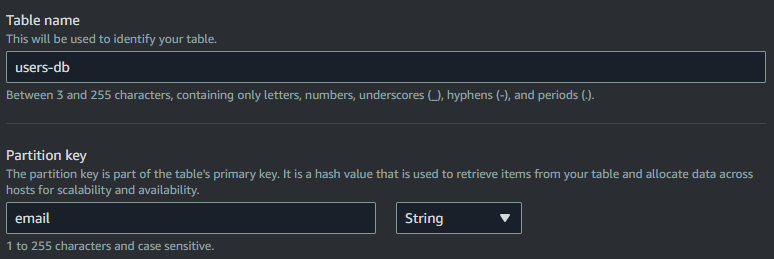
\includegraphics[width = 8cm,keepaspectratio]{tableCreation} \newline
		
		\textit{Eigene Darstellung} % Quelle
		\label{fig:tableCreation}
		\end{minipage}
		\end{figure}
	Diese Tabelle sollte danach noch befüllt werden, damit Daten durch die API ausgegeben werden können. Dabei ist einzig das Schema wichtig, da der Inhalt für die Simulation nicht relevant ist. Jetzt kann die API  erstellt werden, mit der die Daten für einen Nutzer (in diesem Fall für die Lambda-Funktion) erreichbar gemacht werden.
	\subsubsection{Die API}
	Der erste Schritt ist die Definition des Datenschema und der Methoden in GraphQL.
	\paragraph{GraphQL}
	Der GraphQL-Code erfüllt zwei verschiedene Aufgaben: \cite{GraphQL2024} Er definiert das Schema der Datenbank: zwar sind in DynamoDB keine Spalten vorgegeben, eine spaltenunabhängige Codierung ist im Rahmen dieses Projekts aber weder semantisch vorteilhaft noch zeitlich realisierbar. Deshalb wird die Tabelle mit den jeweiligen Datentypen vorgegeben:
	
		\begin{figure}[H]
		\centering
		\begin{minipage}[t]{.7\textwidth} % Breite, z.B. 1\textwidth		
		\caption{Datentypen} % Überschrift
		\begin{lstlisting}[style=graphql]
		type User {
		  email: String!
		  name: String!
		  status: Status
		}
		\end{lstlisting}
		\textit{Eigene Darstellung} % Quelle
		\label{fig:datenTypen}
		\end{minipage}
		\end{figure}
	Bezogen auf den Nutzer werden drei Attribute gespeichert: Die email als String, der Name als String und der Status. Dieser ist entweder ``ACTIVE'' oder ``INACTIVE''. Um das zu erreichen muss in GraphQL ein sogenannter ``enum'' erstellt werden. Enums sind Strukturen, die eine Reihe verschiedener Optionen enthalten. Es werden nur Werte akzeptiert, die so auch in der Struktur gespeichert sind (In diesem Fall ACTIVE und INACTIVE). \cite{https://graphql.com/learn/enums/}
	
		\begin{figure}[H]
		\centering
		\begin{minipage}[t]{.7\textwidth} % Breite, z.B. 1\textwidth		
		\caption{Status} % Überschrift
		\begin{lstlisting}[style=graphql]
		enum Status {
		  ACTIVE
		  INACTIVE
		}
		\end{lstlisting}
		\textit{Eigene Darstellung} % Quelle
		\label{fig:status}
		\end{minipage}
		\end{figure}
	
	Zusätzlich dazu werden in GraphQL die Funktionen der API definiert. Den Anforderungen (s.o.) entsprechend muss es drei Funktionen, eine Mutation und zwei Abfragen geben. Die Abfrage ``GetUsers'' benötigt keine Eingabe, da ohne Selektion alle in der Datenbank enthaltenen Einträge ausgegeben werden. Die Abfrage ``GetUser'' hingegen benötigt die E-Mail als Filterparameter, und die Mutation AddUser braucht alle 3 Informationen über den Nutzer. Das muss in der Definition berücksichtigt werden:
	
		\begin{figure}[H]
		\centering
		\begin{minipage}[t]{.7\textwidth} % Breite, z.B. 1\textwidth		
		\caption{Query und Mutation} % Überschrift
		\begin{lstlisting}[style=graphql]
		type Query {
		  getUsers: [User]
		  getUser(email: String!): User
		}
		
		type Mutation {
		  addUser(email: String!, name: String,! status: Status): User
		}
		\end{lstlisting}
		\textit{Eigene Darstellung} % Quelle
		\label{fig:queryAndMutation}
		\end{minipage}
		\end{figure}
	
	
	\paragraph{API-Methoden}
	Für jede API-Methode existiert eine JavaScript-Datei. Die Methoden unterscheiden sich aufgrund ihrer unterschiedlichen Anforderungen.
	\subparagraph{Bibliothek}
	Um Daten aus der Tabelle mit JavaScript zu editieren, wird eine Bibliothek verwendet, in der verschiedene Standard-Operationen enthalten sind, die auf einer DynamoDB-Tabelle ausgeführt werden können. Auf Basis dieser Bibliothek sind dann alle Methoden aufgebaut. Die Bibliothek wird in allen Dateien unter dem gleichen Alias importiert, weshalb der Import kein Teil der Code-Snippets für die Methoden ist, und stattdessen im Folgenden beispielhaft isoliert dargestellt wird. Der Name, mit der die Bilbiothek referenziert wird, ist ``ddb'':\newline
		\begin{figure}[H]
		\centering
		\begin{minipage}[t]{.7\textwidth} % Breite, z.B. 1\textwidth		
		\caption{Import der Bibliothek} % Überschrift
		\begin{minted}[breaklines=true]{javascript}
		import * as ddb from '@aws-appsync/utils/dynamodb'
		\end{minted}
		
		\textit{Eigene Darstellung} % Quelle
		\label{fig:bibliothekImport}
		\end{minipage}
		\end{figure}
	\subparagraph{Aufbau der Dateien}
	Da in allen JavaScript-Dateien jeweils eine API-Funktion definiert wird, ist der grundlegende Aufbau identisch. Die Dateien unterscheiden sich lediglich durch den Inhalt der Methode selbst. 
	Auf den oben beschriebenen Import der Bibliothek folgend wird die Funktion ``request'' definiert. Die Funktion dient der Behandlung der Anfrage, das Resultat der Methode wird als ``result'' in der Kontext-Variable gespeichert. Die Kontext-Variable wird als Input-Parameter in die Methode gegeben und beinhaltet alle relevanten Informationen rund um die Anfrage. Das Resultat hat keinen vorgegbenen Datentyp:\newline
		\begin{figure}[H]
		\centering
		\begin{minipage}[t]{.7\textwidth} % Breite, z.B. 1\textwidth		
		\caption{Methode Request} % Überschrift
		\begin{minted}[breaklines=true]{javascript}
		export function request(ctx) {
		  //handle the request
		  //return the result
		}
		\end{minted}
		
		\textit{Eigene Darstellung} % Quelle
		\label{fig:requestMethode}
		\end{minipage}
		\end{figure}
	
	Nachdem die Abfrage durch die Request-Methode behandelt wurde, muss auch die Ausgabe behandelt werden. Das geschieht über die Funktion ``response''. Sollte keine weitere Mutation des Resultats nötig sein, sieht diese Methode folgendermaßen aus:\newline
		\begin{figure}[H]
		\centering
		\begin{minipage}[t]{.7\textwidth} % Breite, z.B. 1\textwidth		
		\caption{Methode Response} % Überschrift
		\begin{minted}[breaklines=true]{javascript}
		export const response = (ctx) => ctx.result;
		\end{minted}
	
		\textit{Eigene Darstellung} % Quelle
		\label{fig:responseMethode}
		\end{minipage}
		\end{figure}\newpage
	Der Eingabe-Parameter für die Methode ist ctx, also die Kontext-Variable. Ausgegeben wird ctx.result, die Variable in der das Resultat gespeichert wird. Ist ctx.result leer, so wird ``undefined'' zurückgegeben. Die Methode ist also äquivalent zu der Folgenden:\newline
		\begin{figure}[H]
		\centering
		\begin{minipage}[t]{.7\textwidth} % Breite, z.B. 1\textwidth		
		\caption{Alternative Methode Response} % Überschrift
		\begin{minted}[breaklines=true]{javascript}
		export const response = (ctx) => {
		    if (ctx != null) return ctx.result;
		    else return undefined;
		};
		\end{minted}
	
		\textit{Eigene Darstellung} % Quelle
		\label{fig:alternativeResponseMethode}
		\end{minipage}
		\end{figure}
		\subsubsection{GetUser}
		
	Aus den Anforderungen an diese Methode geht hervor, dass zu den Eingabe-Parametern die email gehören muss, damit nach dieser gefiltert werden kann. Zusätzlich muss noch die Möglichkeit geboten werden, bis zu drei weitere Variablen mitzugeben. Diese stellen dann die Felder dar, die von der API zurückgegeben werden. Für die Ausgabe muss definiert werden, welche Operation ausgeführt wird. Die Antwort ist dann die Rückgabe der Abfrage mit dem Filterparameter:\newline
	
		\begin{figure}[H]
		\centering
		\begin{minipage}[t]{.7\textwidth} % Breite, z.B. 1\textwidth		
		\caption{Methoden GetUser} % Überschrift
		\begin{minted}[breaklines=true]{javascript}
		export function request(ctx) {
		  return ddb.get({ key: { email: ctx.args.email } });
		}
		
		export const response = (ctx) => ctx.result;
		
		\end{minted}
		
		\textit{Eigene Darstellung} % Quelle
		\label{fig:getUserMethoden}
		\end{minipage}
		\end{figure}
	Für die Abfrage wird die Methode ddb.get() verwendet, welche die entsprechend passenden Einträge für einen gegebenen Schlüsselparameter liefert, sofern diese vorhanden sind.
	\subparagraph{GetUsers}
	Aus den Anforderungen an diese Methode geht hervor, dass als Eingabe-Parameter nur die Möglichkeit bestehen muss, die auszugebenden Felder auszuwählen. Für die Ausgabe muss aber definiert werden, welche Operation ausgeführt wird. Die resultierende Antwort ist die Rückgabe der Abfrage:\newline
		\begin{figure}[H]
		\centering
		\begin{minipage}[t]{.7\textwidth} % Breite, z.B. 1\textwidth		
		\caption{Methoden GetUsers} % Überschrift
		\begin{minted}[breaklines=true]{javascript}
		export function request(ctx) {
		  return { operation: 'Scan' };
		}
		
		export const response = (ctx) => ctx.result.items;
		
		\end{minted}
		
		\textit{Eigene Darstellung} % Quelle
		\label{fig:getUsersMethoden}
		\end{minipage}
		\end{figure}
	Aufgrund eines Fehlers mit der Methode ddb.scan() wird hier die Bibliothek nicht eingesetzt. Stattdessen wird die Scan-Operation manuell aufgerufen, und das Ergebnis dieser zurückgegeben. Die Antwort wird dann aus allen Items der ctx-result-Variable gebildet.
	\subparagraph {AddUser}
	Aus den Anforderungen an diese Methode geht hervor, dass als Eingabe-Parameter zumindest die email, also der Schlüssel der Tabelle, gegeben sein muss. Dazu muss die Möglichkeit bestehen, Inhalt für alle anderen Spalten mitzugeben, und Spalten zur Ausgabe auszuwählen. Die Ausgabe bei dieser Mutation ist das durch die Methode selbst hinzugefügte Element:
		\begin{figure}[H]
		\centering
		\begin{minipage}[t]{.7\textwidth} % Breite, z.B. 1\textwidth		
		\caption{Methoden AddUser} % Überschrift
		\begin{minted}[breaklines=true]{javascript}
		export function request(ctx) {
		  const { email, ...values} = ctx.args
		  return {
		    operation: 'PutItem',
		    key: util.dynamodb.toMapValues({email}),
		    attributeValues: util.dynamodb.toMapValues(values),
		  };
		}
		export const response = (ctx) => ctx.result;
		\end{minted}
		
		\textit{Eigene Darstellung} % Quelle
		\label{fig:addUserMethoden}
		\end{minipage}
		\end{figure}
	Zuerst werden hier die Argumente extrahiert, da diese gesondert genutzt werden. Dafür wird ctx.args, die Variable in der alle Argumente gespeichert sind, auf zwei Variablen verteilt. Das erste Argument (in diesem Fall die email als Schlüssel) wird auf die Variable email übertragen, alle weiteren Argumente auf die Liste values. Danach wird die Operation definiert, hier ``PutItem'', also das Hinzufügen eines Elements, woraufhin die Schlüsselspalte und die anderen Spalten auf die vorher gespeicherten Variablen gesetzt werden. Die Response-Methode ist identisch zu der, die in GetUser verwendet wurde.\newline
	Damit aber die API auch abrufbar ist, muss das Backend gehandhabt sein. Dafür ist Terraform zuständig.
	\subsubsection{Terraform}
	Die Basis der in Terraform definierten Infrastruktur ist die Verbindung mit der Datenbank und die Definition der zu verwendenden Rollen für die jeweiligen Abfragen. 
	\paragraph{Definition der Tabelle}
	Zuerst wird dafür eine Resource erstellt, in welcher die von Terraform angeforderten Informationen über die Datenbank angegeben werden. \newline \cite{TerraformBestPractices2024}\newline Dazu gehören der Name der Datenbank, der Zahlungsmodus und der Datenbankschlüssel. Beim Zahlungsmodus unterscheidet AWS zwischen ``provisioned'' und ``pay per request''. Bei unvorhersehbaren Anfragefrequenzen empfiehlt AWS ``pay per request'', weshalb dieses auch hier verwendet wird: Da die Umsetzung auf  dem Testsystem stattfindet, ist nicht von regelmäßiger Nutzung auszugehen. Der Name der Datenbank ist ``users-db'' und der Datenbankschlüssel ist die E-Mail. Mit diesen Informationen kann nun die Ressource erstellt werden:
	
		\begin{figure}[H]
		\centering
		\begin{minipage}[t]{.7\textwidth} % Breite, z.B. 1\textwidth		
		\caption{Definition der Tabelle} % Überschrift
		\begin{minted}[breaklines=true]{terraform}
		resource "aws_dynamodb_table" "user" {
		  name         = "user-db"
		  billing_mode = "PAY_PER_REQUEST"
		  hash_key     = "email"
		
		  attribute {
		    name = "email"
		    type = "S"
		  }
		}
		
		\end{minted}
		
		\textit{Eigene Darstellung} % Quelle
		\label{fig:tabellenDefinition}
		\end{minipage}
		\end{figure}
	\paragraph{Definition der Berechtigungen}
	Da die API zwei verschiedene Methoden-Typen anbietet, die jeweils verschiedene Zugriffslevel benötigen, müssen auch zwei verschiedene Zugriffspolitiken aufgesetzt werden. Für Queries muss die API Daten aus der Tabelle lesen können, und für die Mutation die Tabelle editieren. Die beiden Zugriffsberechtigungen sind vom Aufbau her gleich, weshalb im Folgenden nur zur Veranschaulichung der Schreib-Zugriff beschrieben wird. Die Basis bildet hier ein ``IAM policy document''. Dieses JSON-Dokument enthält Informationen, ohne die der Zugriff nicht gewährt werden kann, und bildet somit die Quelle des Zugriffs. Zusätzlich zu dieser Quelle müssen manuell die Aktionen definiert werden, die mit dieser Rolle verbunden sein sollen, und es muss eine Identifikationsnummer für die Rolle vergeben werden. Diese Informationen werden als Datenobjekt abgespeichert, und können dann von der API zur Authorisierung verwendet werden:
	\newline
	\newline
		\begin{figure}[H]
		\centering
		\begin{minipage}[t]{.7\textwidth} % Breite, z.B. 1\textwidth		
		\caption{Definition der Berechtigungen} % Überschrift
		\begin{minted}[breaklines=true]{terraform}
		data "aws_iam_policy_document" "user_table_write" {
		  source_policy_documents = [data.aws_iam_policy_document.user_table_read.json]
		
		  statement {
		    sid = "WriteItems"
		    actions = [
		      "dynamodb:PutItem",
		      "dynamodb:UpdateItem",
		      "dynamodb:DeleteItem",
		    ]
		    resources = [aws_dynamodb_table.user.arn]
		  }
		}
		
		\end{minted}
		
		\textit{Eigene Darstellung} % Quelle
		\label{fig:berechtigungsDefinition}
		\end{minipage}
		\end{figure}
	\paragraph{Definition der Funktions-Resolver}
	Für jede Funktion der API muss in Terraform ein sogenannter Resolver angelegt werden. In einem Resolver sind Informationen über die Methode hinterlegt, die ausgeführt werden soll. Enthalten muss ein Resolver den Typ der Funktion, die Idenfikationsnummer der API, die Datengrundlage, den Namen der Funktion, die Art der Funktion, und die Datei, in der die Methode beschrieben wird. Im Rahmen dieser Praxisarbeit sind die Methoden in Javascript definiert\footnote{Die Sprache hat keinen Einfluss auf die Funktionsweise, die Entscheidung beruht ausschließlich auf der Präferenz der Entwickler}. Zuletzt muss noch die Runtime der Sprache, in der die Methoden verfasst sind, definiert werden, damit die Methoden ausgeführt werden können. Der Resolver wird dann als Resource abgespeichert. Beispielhaft ist hier die Methode AddUser dargestellt:
	
		\begin{figure}[H]
		\centering
		\begin{minipage}[t]{.7\textwidth} % Breite, z.B. 1\textwidth		
		\caption{Definition der Funktions-Resolver} % Überschrift
		\begin{minted}[breaklines=true]{terraform}
		resource "aws_appsync_resolver" "add_user" {
		  type        = "Mutation"
		  api_id      = aws_appsync_graphql_api.user.id
		  data_source = aws_appsync_datasource.user_table.name
		  field       = "addUser"
		  kind        = "UNIT"
		  code        = file("${path.module}/templates/addUser.js")
		
		  runtime {
		    name            = "APPSYNC_JS"
		    runtime_version = "1.0.0"
		  }
		}
		
		\end{minted}
		
		\textit{Eigene Darstellung} % Quelle
		\label{fig:resolverDefinition}
		\end{minipage}
		\end{figure}
	\paragraph{Aktivierung des Cloud-Watch-Loggings}
	Um das Sammeln von Daten in CloudWatch zu aktivieren, muss eine Methode in Terraform auf die entsprechende Policy referenzieren
	\newline
	\newline
		\begin{figure}[H]
		\centering
		\begin{minipage}[t]{.7\textwidth} % Breite, z.B. 1\textwidth		
		\caption{Aktivierung des Cloud-Watch-Loggings} % Überschrift
		\begin{minted}[breaklines=true]{terraform}
		resource "aws_iam_role_policy_attachment" "logging" {
		  policy_arn = "arn:aws:iam::aws:policy/service-role/AWSAppSyncPushToCloudWatchLogs"
		  role           = aws_iam_role.logging.name
		}
		\end{minted}
		
		\textit{Eigene Darstellung} % Quelle
		\label{fig:loggingAktivierung}
		\end{minipage}
		\end{figure}
	Damit ist der Abruf von Daten gewährleistet. Nun muss das Verteilen von Daten ermöglicht werden.

\subsection{Umsetzung des Datentransports}
	Damit nun erhobenen Daten über die erstellte API verteilt werden können, muss die Infrastruktur für die Verteilung der Daten aufgebaut werden:
	\subsubsection{AWS-Datadog-Integration}
	Die praktische Umsetzung der Integration beschränkt sich auf die Eingabe von Daten in die Benutzeroberflächen von DataDog und AWS.
	\paragraph{DataDog}
	Zuerst muss in DataDog ein neuer AWS-Account als Integration hinzugefügt werden. Dabei werden dem Nutzer vier Anpassungsoptionen gegeben:\newline
	1. AWS-Region\newline
	In diesem Fall, da die Auftraggebende Abteilung auf diesem Server beheimatet ist, ist die Region ``eu-central-1''\newline
	2. API Key\newline
	Lässt der Nutzer hier das Feld unverändert, generiert DataDog automatisch einen API-Key. Für dieses Projekt wurde bereits im Vorfeld ein API-Key angelegt, der deshalb hier ausgewählt wird.\newline
	3. AWS Logs senden\newline
	Damit die im vorigen Kapitel aufgesetzten Lambda-Funktionen einen Nutzen haben, sollte diese Option aktiviert sein.\newline
	4. Cloud Security Verwaltung anschalten\newline
	Im Rahmen dieser Praxisarbeit ist Sicherheit nicht ausschlaggebend, da keine schützenswerten Daten behandelt werden. Die Kosten für Sicherheit werden dementsprechend gespart und diese Option bleibt deaktiviert.\newline
	\newline
	Nachdem die Felder ausgefüllt wurden, kann das Template erstellt werden. Damit ist der in DataDog zu absolvierende Teil abgeschlossen. \newline
	\paragraph{AWS}
	Mit der Fertigstellung des Templates in DataDog wird der Nutzer automatisch in die Applikation ``CloudFormation'' weitergeleitet. Dort kann dann mit dem API-Key aus DataDog und einem App-Key, welcher ebenfalls in DataDog generiert wird, ein Stack erstellt werden. Damit ist die Verbindung abgeschlossen und Daten können zwischen AWS und DataDog fließen.
\subsection{Umsetzung des Datenabrufs}
	Im Rahmen der Lambda-Funktionen werden drei verschiedene Dateien verwendet. In der Datei ``shared.py'' sind die Methoden hinterlegt, die für alle Funktionen relevant sind. Die Dateien ``success.py'' und ``error.py'' beinhalten jeweils eine Lambda-Funktion, wobei erstere eine korrekte, und zweitere eine fehlerhafte Anfrage simuliert. 
	\paragraph{Geteilte Methoden}
		Für die Funktionen werden drei verschiedene unterstützende Methoden benötigt (in diesem speziellen Anwendungsfall, diese Zahl ist nicht unbedingt auf andere Projekte übertragbar). Mit einer Methode wird die Instanz eines 		sogenannten ``logger''s verteilt. Ein logger ist dafür zuständig, Nachrichten über die Ausführung eines Programms auszugeben:\newline
		\begin{figure}[H]
		\centering
		\begin{minipage}[t]{.7\textwidth} % Breite, z.B. 1\textwidth		
		\caption{GetLogger-Methode} % Überschrift
		\begin{minted}[breaklines=true]{python}
		def get_logger(level: int = logging.INFO):
		    logger = logging.getLogger()
		    logger.setLevel(level)
		    return logger
		\end{minted}
		
		\textit{Eigene Darstellung} % Quelle
		\label{fig:getLoggerMethode}
		\end{minipage}
		\end{figure}
	Eine weitere Methode ist dafür zuständig, das API-Secret zu generieren, mit welchem sich die Methoden authentifizieren:\newline
		\begin{figure}[H]
		\centering
		\begin{minipage}[t]{.7\textwidth} % Breite, z.B. 1\textwidth		
		\caption{GetSecret-Methode} % Überschrift
		\begin{minted}[breaklines=true]{python}
		def get_secret(secret_id: str) -> str:
		    response = sm_client.get_secret_value(SecretId=secret_id)
		    return response["SecretString"]
		\end{minted}
		
		\textit{Eigene Darstellung} % Quelle
		\label{fig:getSecretMethode}
		\end{minipage}
		\end{figure}
	Die letzte Methode ist dafür zuständig die Query auszuführen, die in den beiden anderen Dateien definiert wird. Als Eingabe-Parameter werden die URL der angesprochenen Schnittstelle, der API-Key und die query erwartet:\newline
		\begin{figure}[H]
		\centering
		\begin{minipage}[t]{.7\textwidth} % Breite, z.B. 1\textwidth		
		\caption{Query-Methode} % Überschrift
		\begin{minted}[breaklines=true]{python}
		def query(url: str, key: str, query: str):
		\end{minted}
		
		\textit{Eigene Darstellung} % Quelle
		\label{fig:queryMethode}
		\end{minipage}
		\end{figure}
	Die Bearbeitung ist in mehrere Schritte gegliedert:\newline
	1. Definition der query:\newline
		\begin{figure}[H]
		\centering
		\begin{minipage}[t]{.7\textwidth} % Breite, z.B. 1\textwidth		
		\caption{Definition der Query} % Überschrift
		\begin{minted}[breaklines=true]{python}
		data = json.dumps({"query": query}).encode()
		\end{minted}
		
		\textit{Eigene Darstellung} % Quelle
		\label{fig:queryDefinition}
		\end{minipage}
		\end{figure}
	2. Formierung des requests, indem das Request selbst mit Methode und URL und der Header mit Content-Type und API-Key definiert werden:\newline
		\begin{figure}[H]
		\centering
		\begin{minipage}[t]{.7\textwidth} % Breite, z.B. 1\textwidth		
		\caption{Formierung des Requests} % Überschrift
		\begin{minted}[breaklines=true]{python}
		req = request.Request(url, method="POST")
		    req.add_header("x-api-key", key)
		    req.add_header("Content-Type", "application/graphql")
		\end{minted}
		
		\textit{Eigene Darstellung} % Quelle
		\label{fig:requestFormierung}
		\end{minipage}
		\end{figure}
	3. Durchführung der Anfrage und Rückgabe der Antwort:\newline
		\begin{figure}[H]
		\centering
		\begin{minipage}[t]{.7\textwidth} % Breite, z.B. 1\textwidth		
		\caption{Durchführung der Anfrage} % Überschrift
		\begin{minted}[breaklines=true]{python}
		response = request.urlopen(req, data=data)
		return json.loads(response.read())
		\end{minted}
		
		\textit{Eigene Darstellung} % Quelle
		\label{fig:anfrageDurchführung}
		\end{minipage}
		\end{figure}
	\paragraph{Simulation der fehlerhaften Abfrage}
	Basis der fehlerhaften Anfrage ist eine fehlerhafte Query. Diese sieht folgendermaßen aus:\newline
		\begin{figure}[H]
		\centering
		\begin{minipage}[t]{.7\textwidth} % Breite, z.B. 1\textwidth		
		\caption{Fehlerhafte Query} % Überschrift
		\begin{minted}[breaklines=true]{python}
		QUERY = """
		query MyQuery {
		  getUsers {
		    email
		    name
		    stat
		  }
		}
		"""
		\end{minted}
		
		\textit{Eigene Darstellung} % Quelle
		\label{fig:fehlerhafteQuery}
		\end{minipage}
		\end{figure}
	Das Feld ``stat'' existiert nicht, weshalb hier in der Ausführung ein Fehler ausgeworfen wird. 
	\newline
	Zusätzlich beinhaltet die Datei eine Methode, mit der die Query behandelt wird. Diese teilt sich folgendermaßen auf:\newline
	1. Generieren des API-Keys mithilfe der get secret-Methode aus ``shared.py'':\newline
		\begin{figure}[H]
		\centering
		\begin{minipage}[t]{.7\textwidth} % Breite, z.B. 1\textwidth		
		\caption{Generieren des API-Keys} % Überschrift
		\begin{minted}[breaklines=true]{python}
		key = get_secret(os.environ["API_KEY_SECRET_ID"])
		\end{minted}
		
		\textit{Eigene Darstellung} % Quelle
		\label{fig:apiKeyGenerierung}
		\end{minipage}
		\end{figure}
	2. Ausführen der Query über die Methode aus  ``shared.py'':\newline
		\begin{figure}[H]
		\centering
		\begin{minipage}[t]{.7\textwidth} % Breite, z.B. 1\textwidth		
		\caption{Ausführen der Query} % Überschrift
		\begin{minted}[breaklines=true]{python}
		result = query(os.environ["API_URL"], key, QUERY)
		\end{minted}
		
		\textit{Eigene Darstellung} % Quelle
		\label{fig:queryAusführung}
		\end{minipage}
		\end{figure}
	3. Generieren des loggers mithilfe der Methode aus ``shared.py'' und Dokumentation des Fehlers:\newline
		\begin{figure}[H]
		\centering
		\begin{minipage}[t]{.7\textwidth} % Breite, z.B. 1\textwidth		
		\caption{Generieren des Loggers} % Überschrift
		\begin{minted}[breaklines=true]{python}
		get_logger().error(result)
		\end{minted}
		
		\textit{Eigene Darstellung} % Quelle
		\label{fig:loggerGenerierung}
		\end{minipage}
		\end{figure}
	4. Rückgabe des Felds ``errors'' aus dem Resultat:\newline
		\begin{figure}[H]
		\centering
		\begin{minipage}[t]{.7\textwidth} % Breite, z.B. 1\textwidth		
		\caption{Rückgabe des Felds ``errors''} % Überschrift
		\begin{minted}[breaklines=true]{python}
		return result["errors"]
		\end{minted}
		
		\textit{Eigene Darstellung} % Quelle
		\label{fig:errorFeldRückgabe}
		\end{minipage}
		\end{figure}
	\paragraph{Simulation der erfolgreichen Abfrage}
	Basis der erfolgreichen Abfrage ist eine korrekte Query. Diese sieht folgendermaßen aus:\newline
		\begin{figure}[H]
		\centering
		\begin{minipage}[t]{.7\textwidth} % Breite, z.B. 1\textwidth		
		\caption{Korrekte Query} % Überschrift
		\begin{minted}[breaklines=true]{python}
		QUERY = """
		query MyQuery {
		  getUsers {
		    email
		    name
		    status
		  }
		}
		"""
		\end{minted}
		
		\textit{Eigene Darstellung} % Quelle
		\label{fig:korrekteQuery}
		\end{minipage}
		\end{figure}
	Genau wie die Simulation der fehlerhaften Abfrage wird die Query auch hier in einer seperaten Methode behandelt. Diese ist bis auf die Rückgabe identisch. Zurückgegeben wird nicht der Fehler sondern das korrekte Resultat:\newline
		\begin{figure}[H]
		\centering
		\begin{minipage}[t]{.7\textwidth} % Breite, z.B. 1\textwidth		
		\caption{Rückgabe des korrekten Resultats} % Überschrift
		\begin{minted}[breaklines=true]{python}
		return result["data"]["getUsers"]
		\end{minted}
		
		\textit{Eigene Darstellung} % Quelle
		\label{fig:resultatsRückgabe}
		\end{minipage}
		\end{figure}
Jetzt ist ein Datenabruf in externen Anwendungen möglich. Der letzte Schritt ist jetzt, die Daten in ebendiesen Anwendungen auszuwerten.
\subsection{Umsetzung des Daten-Monitorings}
Zuerst soll die Stabilität der API kontrolliert werden. Das soll über ein DataDog-Dashboard geschehen.
\subsubsection{DataDog}
Aus den Anforderungen gehen drei verschiedene zu implementierende Module hervor. Das erste ist ein Zeitstrahl, mit dem die Response time im zeitlichen Kontext dargestellt werden kann.  Das andere ist ein Diagramm, durch welches eine Relation zwischen erfolgreichen und nicht erfolgreichen Abfragen hergestellt werden kann. Hier bietet sich ein Tortendiagramm an, ein Balkendiagramm, Strahlendiagramm oder aber auch ein Zeitstrahl für Tendenzen wären denkbar. Die Auswahl basiert hier nicht darauf, welches Diagramm am besten für den Nutzungsfall geeignet ist. Schließlich ist diese Entscheidung auch von Nutzerpräferenzen abhängig, und kann aufgrund des frühen Entwicklungsstadiums noch nicht miteinbezogen werden kann.
\paragraph{Zeitstrahl}
Für den Zeitstrahl wird die Metrik ``aws.appsync.latency'' verwendet. Ein Strahl stellt dabei die exakte Response time zu einem bestimmten Zeitpunkt dar, während der andere die zugehörige Trendlinie bildet, die das Visualisieren von Trends vereinfachen soll:\newline

	\begin{figure}[H]
	\centering
	\begin{minipage}[t]{.7\textwidth} % Breite, z.B. 1\textwidth		
	\caption{Zeitstrahl; Einstellungen} % Überschrift
	
	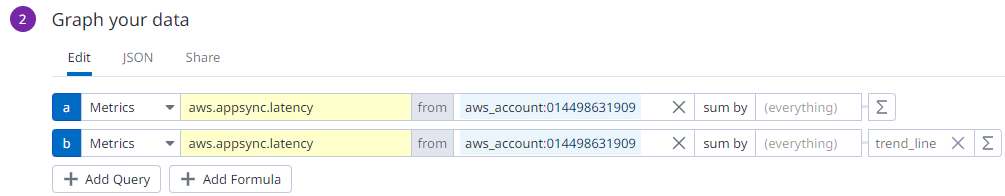
\includegraphics[width = 10cm,keepaspectratio]{graphOneSettings}\newline
	\textit{Eigene Darstellung} % Quelle
	\label{fig:zeitStrahlEinstellungen}
	\end{minipage}
	\end{figure}
	
	Hier ein beispielhafter Ausschnitt des Graphen:
	
	\begin{figure}[H]
	\centering
	\begin{minipage}[t]{.7\textwidth} % Breite, z.B. 1\textwidth		
	\caption{Zeitstrahl} % Überschrift
	
	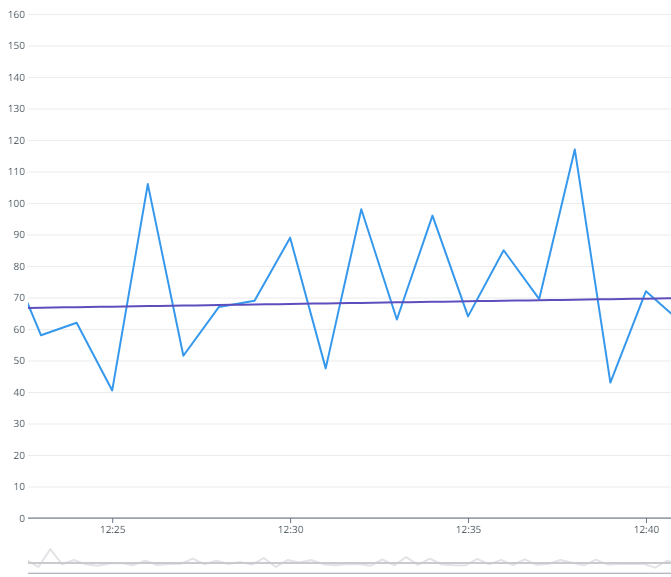
\includegraphics[width = 8cm,keepaspectratio]{graphOneItself} \newline
	
	\textit{Eigene Darstellung} % Quelle
	\label{fig:zeitstrahl}
	\end{minipage}
	\end{figure}
 
\paragraph{Tortendiagramm}
Zur Umsetzung des Tortendiagramms müssen die Filter so gewählt werden, dass mit einer einzigen OR-Abfrage informative logs von fehlerhaften und erfolgreichen Abfragen (im Folgenden Antworten) unterschieden werden können. Unter anderem unterscheiden sich die beiden JSONs der Antwort-Logs von den informativen logs darin, dass in Informativen Logs kein Event existiert. Die variable ``evt.name'' existiert nur in Antwort-Logs. Der Filter wird also folgendermaßen aufgebaut: \newline
\begin{figure}[H]
\centering
	\begin{minipage}[t]{.7\textwidth} % Breite, z.B. 1\textwidth		
	\caption{Tortendiagramm Filter} % Überschrift
	
	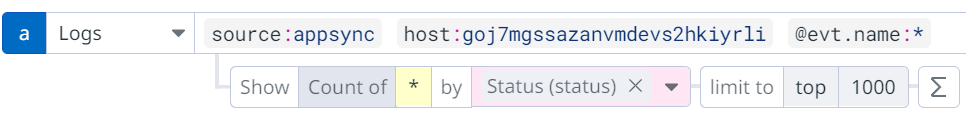
\includegraphics[width = 8cm,keepaspectratio]{pieChartFilter} \newline
	
	\textit{Eigene Darstellung} % Quelle
	\label{fig:pieChartFilter}
	\end{minipage}
	\end{figure}
Es sollen nur Logs der API, an der dieses Projekt durchgeführt wird, und von AppSync gesendet wurden, in dieses Tortendiagram einfließen. Das stellen die ersten beiden Filter sicher. Danach wird ein sogenannter Wildcard-Filter auf das Feld ``evt.name'' angewendet. Das bedeutet, dass alle Logs in dieses Diagramm einfließen, die irgendeinen Wert für dieses Feld haben. Da das Feld nur für Antwort-Logs existiert, werden dadurch alle informativen Logs herausgefiltert, und das gewünschte Diagramm erreicht:\newline

	\begin{figure}[H]
	\centering
	\begin{minipage}[t]{.7\textwidth} % Breite, z.B. 1\textwidth		
	\caption{Tortendiagramm} % Überschrift
	
	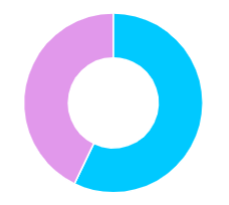
\includegraphics[width = 8cm,keepaspectratio]{pieChart} \newline
	
	\textit{Eigene Darstellung} % Quelle
	\label{fig:pieChart}
	\end{minipage}
	\end{figure}
\subsubsection{CloudWatch}
Aus dem DataDog-Dashboard lässt sich, sollte der Bedarf bestehen, zu jedem Log eines Fehlers der jeweilige logStream herauslesen:\newline

	\begin{figure}[H]
	\centering
	\begin{minipage}[t]{.7\textwidth} % Breite, z.B. 1\textwidth		
	\caption{LogStream} % Überschrift
	
	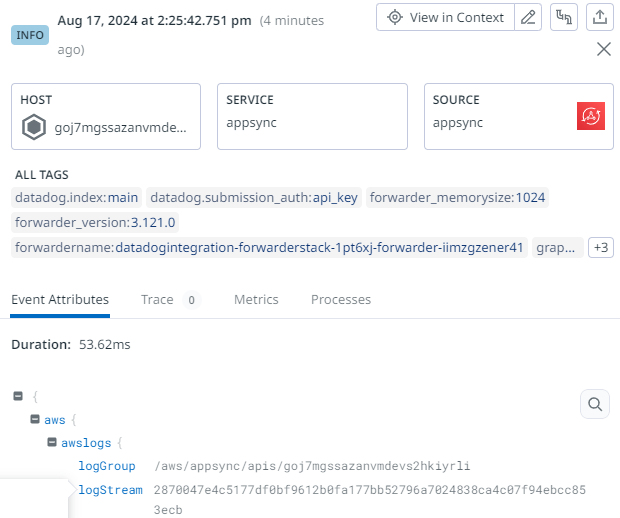
\includegraphics[width = 8cm,keepaspectratio]{logStream} \newline
	
	\textit{Eigene Darstellung} % Quelle
	\label{fig:logStream}
	\end{minipage}
	\end{figure}
 
Mit dieser Identifikationsnummer kann dann auf den LogStream in CloudWatch zugegriffen werden, in welchem alle Informationen zu dem Fehler aufzufinden sind. Das ist möglich, indem innerhalb der LogStream-Sammlung der API mithilfe der Identifikationsnummer gefiltert wird:\newline

	\begin{figure}[H]
	\centering
	\begin{minipage}[t]{.7\textwidth} % Breite, z.B. 1\textwidth		
	\caption{Filter für den LogStream} % Überschrift
	
	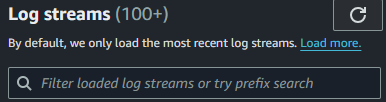
\includegraphics[width = 8cm,keepaspectratio]{logStreamFilter} \newline
	
	\textit{Eigene Darstellung} % Quelle
	\label{fig:logStreamFilter}
	\end{minipage}
	\end{figure}
 
Hier ein beispielhafter Ausschnitt aus den Logs:
	\begin{figure}[H]
	\centering
	\begin{minipage}[t]{.7\textwidth} % Breite, z.B. 1\textwidth		
	\caption{LogStream Beispiel} % Überschrift
	
	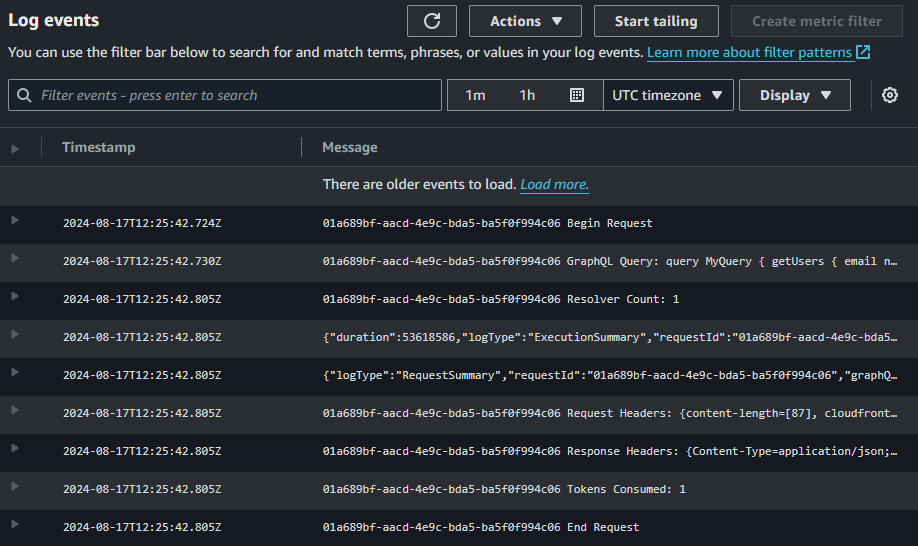
\includegraphics[width = 8cm,keepaspectratio]{logStreamExample} \newline
	
	\textit{Eigene Darstellung} % Quelle
	\label{fig:logStreamBeispiel}
	\end{minipage}
	\end{figure}
 
Durch die Informationen, die aus diesen Logs hervorgehen (Fehlertyp, Stelle im Code/in der Abfrage), wird das Debuggen der Fehler erleichtert. 
\section{Fazit} 
\subsection{Bedeutung für das Unternehmen}
Da diese Umsetzung sich auf eine Testumgebung beschränkt, entspringt aus der Arbeit für das Unternehmen kein direkter wertschöpfender Nutzen. Die Infrastruktur, die im Rahmen dieser Praxisarbeit aufgebaut wurde, wird aber, sobald sie auf das Produktiv-System übertragen wird, einen großen positiven Einfluss auf die Maintainability der APIs haben. 
\subsection{Bewertung des Erreichens der Zielstellung}
Um das Erreichen der Zielstellung zu evaluieren, werden im Folgenden die vier in den Anforderungen definierten Erwartungen bewertet.
\subsubsection{Erstellung der Datengrundlage}
Die Datengrundlage ist in Form der DynamoDB-Tabelle vollständig funktionsfähig erstellt. Ebenso vollständig funktionsfähig ist die API und das zugehörige Terraform-Backend. Alle angeforderten Funktionen sind hier vollständig abgedeckt
\subsubsection{Datentransport}
Die für den Datentransport benötigte Infrastruktur ist vollständig aufgebaut; Daten können zwischen allen Anwendungen fließen, bei denen ein Datenfluss vorgesehen war. 
\subsubsection{Datenabruf}
Die Lambda-Funktionen, mit denen API-Anfragen automatisch generiert werden, funktionieren fehlerfrei. 
\subsubsection{Daten-Monitoring}
Das DataDog-Dashboard enthält alle in den Anforderungen vorgesehene Funktionen. Insofern sind die Anforderungen erfüllt, wenngleich weitere Entwicklung mit Einbezug von Nutzerfeedback nötig ist, um das Dashboard als vollständig werten zu können.\newline
Da in CloudWatch keine zusätzliche Entwicklung nötig war, ist die Funktionsweise vorhersehbar. In den Anforderungen wurden nur Funktionen beschrieben, die von CloudWatch abgedeckt werden können.
\newline
Insgesamt wurde, gemäß der Zielstellung, eine Infrastruktur erstellt, mit der die Effizienz und Effektivität einer API im AWS-System verbessert werden kann.
\subsection{Ausblick}
Die Übertraung der im Rahmen dieser Praxisarbeit erarbeiteten Infrastruktur auf das Produktiv-System steht in Zukunft im Mittelpunkt. Entsprechende Anpassungen werden vor allem bezüglich der Lambda-Funktion und des Terraform-Backends nötig sein, da die Datenstruktur nicht identisch ist. Erweiterungen der bereits erstellten Infrastruktur können je nach Nutzer-Rückmeldungen durchgeführt werden; erwartet sind diese hauptsächlich im DataDog-Dashboard.y

	
%%%%%%%%%%%%%%%%%%%%%%%%%%%%%%%%%%%%%%%%%%%%%%%%%%%%%%%%%%%%%%%%%%%%%%%

%%!TEX root = ../Thesis.tex
\section*{Anhang}
\addcontentsline{toc}{section}{Anhang}
\fancyhead[R]{Anhang}

\anhangsverzeichnis

%!TEX root = ../Thesis.tex
\section*{Quellenverzeichnis}
\addcontentsline{toc}{section}{Quellenverzeichnis}
\fancyhead[R]{Quellenverzeichnis}

\defbibheading{mono}{\subsection*{Monographien}}
\defbibheading{mag}{\subsection*{Aufsätze in Sammelbänden und Zeitschriften}}
\defbibheading{art}{\subsection*{Zeitungsartikel}}
\defbibheading{web}{\subsection*{Internetquellen}}
\defbibheading{leg}{\subsection*{Rechtsprechung}}
\defbibheading{comp}{\subsection*{Unternehmensunterlagen/Gesprächsnotizen}}

\setlength\bibitemsep{1.5\itemsep}
\setlength{\bibhang}{2em}

\renewcommand{\baselinestretch}{1.50}\normalsize

\begingroup
\sloppy

\printbibliography[heading=mono,keyword=mono]
\printbibliography[heading=mag,keyword=mag]
\printbibliography[heading=web,keyword=web]

% Bei Bedarf einkommentieren: (erzeugt sonst Warnungen)
% \printbibliography[heading=art,keyword=art]
% \printbibliography[heading=leg,keyword=leg]
% \printbibliography[heading=comp,keyword=comp]

\endgroup


%%%%%%%%%%%%%%%%%%%%%%%%%%%%%%%%%%%%%%%%%%%%%%%%%%%%%%%%%%%%%%%%%%%%%%%

%!TEX root = ../Thesis.tex

\section*{Ehrenwörtliche Erklärung}
\addcontentsline{toc}{section}{Ehrenwörtliche Erklärung}
\fancyhead[R]{Ehrenwörtliche Erklärung}

Hiermit erkläre ich, dass ich die vorliegende \dokumententyp{} selbständig angefertigt habe. Es wurden nur die in der Arbeit ausdrücklich benannten Quellen und Hilfsmittel benutzt. Wörtlich oder sinngemäß übernommenes Gedankengut habe ich als solches kenntlich gemacht. Diese Arbeit hat in gleicher oder ähnlicher Form noch keiner Prüfungsbehörde vorgelegen.
\vspace{20mm}

\ort, \abgabedatum
\vspace{10mm}

\underline{\hspace{8cm}}\\\dokumentenautor
 
%%%%%%%%%%%%%%%%%%%%%%%%%%%%%%%%%%%%%%%%%%%%%%%%%%%%%%%%%%%%%%%%%%%%%%%

\end{document}